\section{Proposed Method}
\label{sec:method}

\subsection{Overview: A Two-Layer Architecture}
\label{sec:method-overview}
The proposed system separates inspection into two cooperating layers
(Fig.~\ref{fig:arch}). A \emph{deliberative} layer performs the inspection
patrol: it visits a sequence of waypoints around the equipment using a standard
navigation stack (Nav2 with a Model Predictive Path Integral controller). We
interpret this layer as \emph{active sensing}: a purely reactive agent responds
only to stimuli already within sensor range, so a mechanism is required
\emph{beforehand} to carry the sensors to where events may occur. The patrol
provides exactly that placement.

A \emph{reactive} layer, named \textsc{Stay Alert}, runs on top of
the patrol. It is governed by an attraction--repulsion field $\Phi$ that grows when a
salient sensory event enters range, driving the robot to \emph{approach}
points of interest (positive $\Phi$, e.g., a thermal hotspot or a partial
discharge) or to \emph{retreat} from danger (negative $\Phi$, e.g., an
arc-flash zone). \textsc{Stay Alert} does not replace the planner: while $\Phi$
is neutral the robot follows the patrol; when an event becomes salient,
\textsc{Stay Alert} preempts the current waypoint, issues a focused navigation
goal (an approach or a retreat pose), and returns control to the patrol once
the event has been handled. This decoupling keeps the deliberative guarantees
of a mature stack while adding a fast, interpretable reactive response.
The field $\Phi$ drives the reactive state machine
(Section~\ref{sec:method-stayalert}); the same field can also be written into a
tabular value update, which we record in Appendix~\ref{app:update} as a design note
since it does not select the executed actions. We revisit this distinction in
Section~\ref{sec:results}.

\begin{figure}[t]
\centering
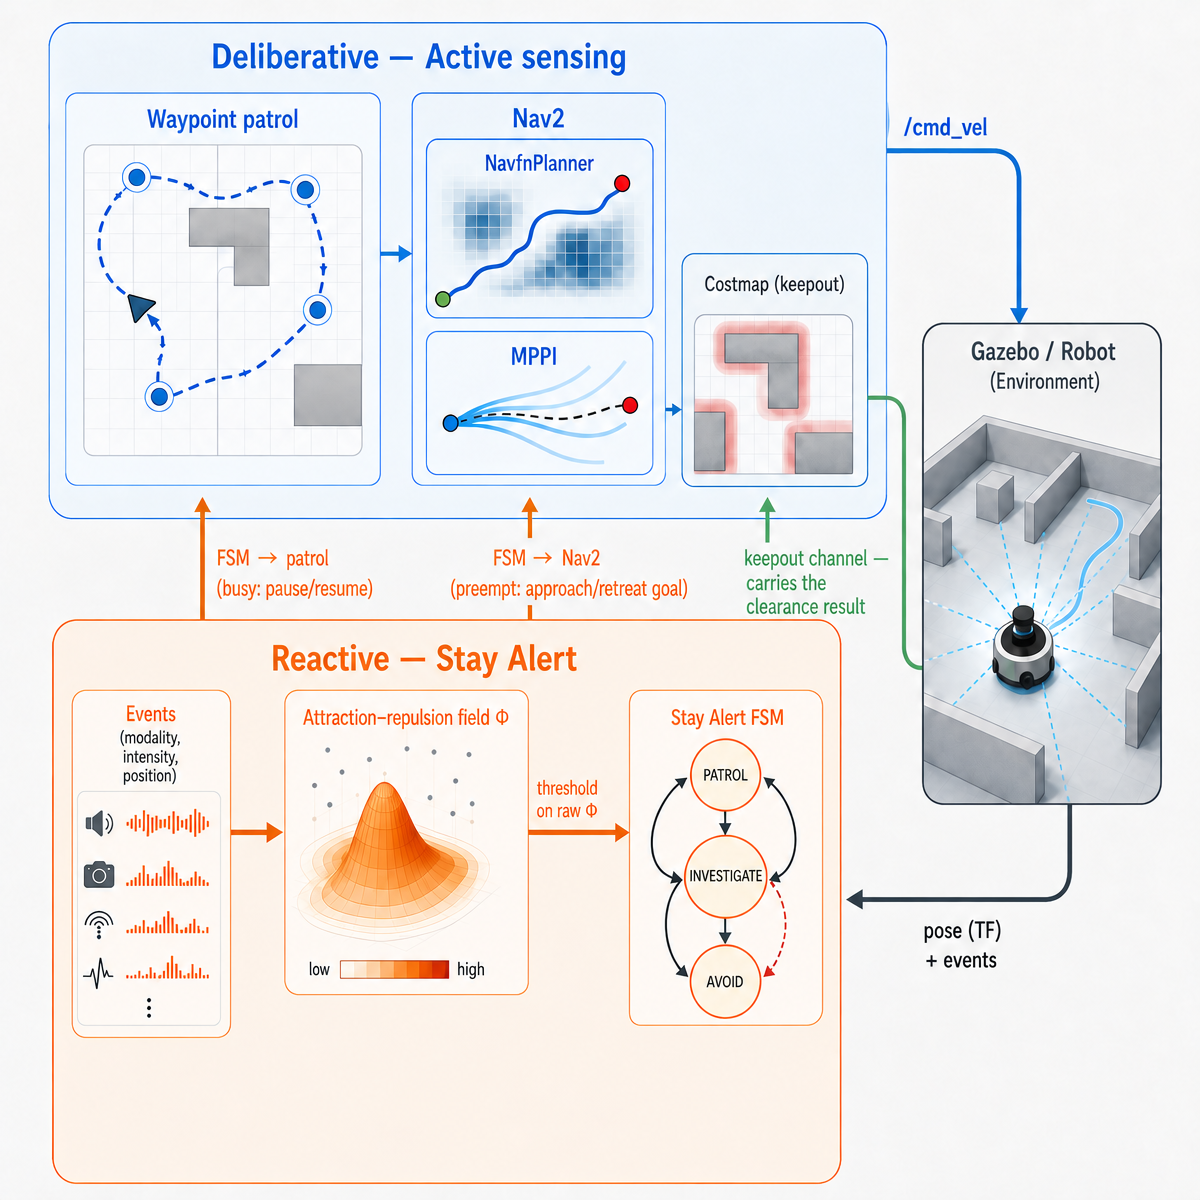
\includegraphics[width=\columnwidth]{architecture}
\caption{Two-layer architecture. The deliberative layer (top) drives a waypoint
patrol through Nav2 (NavfnPlanner $+$ MPPI), sending \texttt{/cmd\_vel} to the
robot. The reactive layer (bottom, \textsc{Stay Alert}) turns sensed
events into the attraction/repulsion field and runs the finite-state machine; it
preempts Nav2 with an approach/retreat goal and pauses/resumes the patrol. The
value update of Appendix~\ref{app:update} is fed by the same field but does not
select the executed actions. The environment returns pose (TF) and events.}
\label{fig:arch}
\end{figure}

\subsection{The Attraction--Repulsion Field}
\label{sec:method-field}
%% R3#1/R2#1 (resubmissão): esta subseção chamava-se "Attractor-Augmented Bellman
%% Update" e abria pela atualização de valor. Como a tabela de valor NÃO seleciona
%% as ações executadas, liderar por ela prometia um componente de aprendizado que o
%% sistema não tem. A subseção passa a definir apenas o que o sistema USA -- o campo
%% e sua arbitragem -- e a formulação da atualização de valor foi movida para o
%% Apêndice~\ref{app:update} como nota de projeto.
The reactive layer is driven by a scalar field $\Phi$ that aggregates the sensory
events at the robot's location---modality, intensity and distance---and carries the
sign of the response: positive for attraction, negative for repulsion. It is a
function of the robot's current observations alone and does not depend on which
action is taken. The field encodes \emph{sensory saliency} and carries the sign of
the response:
\begin{equation}
\label{eq:phi}
\Phi
\begin{cases}
> 0 & \text{attraction (anomaly: approach)}\\
< 0 & \text{repulsion (hazard: retreat)}\\
= 0 & \text{neutral (default patrol behavior).}
\end{cases}
\end{equation}

The field is formed from sensory \emph{events}. An event $e$ of modality
$m\in\{\text{thermal},\text{acoustic},\text{hazard}\}$ at distance $d$ from the
robot is sensed within a detection radius $R$ with intensity
\begin{equation}
\label{eq:intensity}
i_e(d) = I_e\left(1 - \tfrac{1}{2}\,\frac{d}{R}\right), \qquad d \le R,
\end{equation}
$I_e$ being its base intensity. This profile models a \emph{soft detection
boundary}: sensing degrades linearly with range and is not reported beyond $R$.
The resulting step at $d=R$ (from $I_e/2$ to no event) does not induce chattering
of the reactive response, because the controller uses hysteresis---distinct enter
and exit thresholds (Section~\ref{sec:method-stayalert})---and, once it commits to
an event, does not re-select it until the episode ends; an event that lapses at
the boundary therefore cannot repeatedly re-trigger the same maneuver. We further
report the method's sensitivity to perception noise in
Section~\ref{sec:results}. Each modality has a weight $w_m$ (with
$w_{\text{hazard}}<0$ for repulsion) and a trigger threshold $\theta_m$. The
field enforces \emph{safety before inspection} as a \emph{precedence} rule, not a
magnitude contest: whenever any repulsive event is above threshold within range,
$\Phi$ takes its (negative) value; only in the absence of a hazard does the field
select, among the concurrent attraction events, the strongest in magnitude. It
then decays geometrically once the event is no longer observed:
Let $\mathcal{E}_{\mathcal{H}}=\{e:\,m(e)\in\mathcal{H},\ i_e\ge\theta_{m(e)}\}$ and
$\mathcal{E}_{\mathcal{A}}=\{e:\,m(e)\in\mathcal{A},\ i_e\ge\theta_{m(e)}\}$ be the
above-threshold hazard and attraction \emph{events} in range at the current step
(each $e$ carries a modality $m(e)$, intensity $i_e$ and identity). The governing
event and the field are formed by \emph{two decaying accumulators}---a hazard
channel $h\ge 0$ and a signed attraction channel $a$---rather than by a single
instantaneous selection, matching the implementation. Writing $c_e=w_{m(e)}\,i_e$
for the signed contribution of event $e$, each step updates the channels by a
magnitude-preserving max-hold,
\begin{align}
\label{eq:phi-chan}
h &\leftarrow \max\!\big(h,\ \textstyle\max_{e\in\mathcal{E}_{\mathcal{H}}}|c_e|\big),\\
a &\leftarrow c_{e^\star}\ \ \text{when } |c_{e^\star}|>|a|\ \ (\text{else held}),
\end{align}
with $e^\star=\operatorname*{arg\,max}_{e\in\mathcal{E}_{\mathcal{A}}}|c_e|$ and
ties broken by the smallest event identity. Once per decay period both channels
relax geometrically and are floored at a residual $\varepsilon$,
\begin{equation}
\label{eq:phi-decay}
h\leftarrow\lambda h,\qquad a\leftarrow\lambda a\quad(\text{set to }0\text{ if below }\varepsilon).
\end{equation}
Each accumulator is \emph{saturated in place} on update---$h\in[0,\Phi_{\max}]$
and $a\in[-\Phi_{\max},\Phi_{\max}]$---so the stored value, not merely its
reading, is bounded (the decay of Eq.~\eqref{eq:phi-decay} then acts on this
bounded state). The field is read off by \emph{categorical precedence},
\begin{equation}
\label{eq:phi-update}
\Phi=-h\ \ \text{if } h>\varepsilon,\qquad
\Phi=a\ \ \text{otherwise,}
\end{equation}
with decay $\lambda\in(0,1)$, residual $\varepsilon$, decay period $T_d$, and
$\mathcal{H}$, $\mathcal{A}$ indexing the repulsive and attractive modalities; when
a channel's \emph{own} eligible set is empty at a step, that channel is left to the
decay of Eq.~\eqref{eq:phi-decay} while the other may still be updated by its
events. We use $\lambda=0.85$, $T_d=1$~s,
$\varepsilon=10^{-3}$ and $\Phi_{\max}=2$ (Table~\ref{tab:hyper}). This memory has two consequences a purely
instantaneous rule would lack: (i) a \emph{recently observed} hazard keeps
governing the field through its decaying magnitude even when only an attraction is
in range at the current step, until $h$ falls below $\varepsilon$; and (ii) a
weaker current event does not overwrite a stronger stored one until the latter has
decayed. Hazards are considered first, so a hazard channel above $\varepsilon$
always governs the field, independently of a concurrent stronger attraction: the
magnitude contest only ever decides \emph{which anomaly} to approach, never
whether to prefer inspection over safety. The \textsc{Avoid} transition then fires
when this field crosses the supervisor threshold ($\Phi\le-\theta_{\text{in}}$)
\emph{and} a retreat pose is available, the post-retreat refractory has elapsed,
and the reactive retreat is enabled (Algorithm~\ref{alg:stayalert})---not as a
function of hazard range alone. We verify the precedence directly in a conflict
scenario (Section~\ref{sec:conflict}), in which a hazard co-located with a
\emph{stronger} anomaly still preempts inspection.

\subsection{The \textsc{Stay Alert} Reactive Layer}
\label{sec:method-stayalert}
\textsc{Stay Alert} is a finite-state machine with three modes:
\textsc{Patrol}, \textsc{Investigate} (attraction) and \textsc{Avoid}
(repulsion), summarized in Algorithm~\ref{alg:stayalert} and
Fig.~\ref{fig:fsm}. Repulsion has priority over attraction (safety before
inspection) \emph{from any state}: whenever $\Phi \le -\theta_{\text{in}}$ and a
retreat pose is available, the robot enters \textsc{Avoid} and navigates to a
retreat pose---\emph{preempting} an in-progress \textsc{Investigate} (outcome
\emph{deferred})---subject to a short refractory $t_{\text{ref}}$ that prevents
immediate re-triggering while the deliberative keepout (Section~\ref{sec:results})
takes over. Otherwise, from \textsc{Patrol}, if $\Phi \ge \theta_{\text{in}}$ the
layer commits the most salient in-range event and enters \textsc{Investigate},
navigating to its inspection pose. On entering either mode the layer asserts a
\emph{busy} flag that pauses the patrol (the current waypoint goal is cancelled)
and emits an event marker carrying the target's identity.

\textsc{Investigate} terminates \emph{successfully} (outcome \emph{inspected})
only when the reactive navigation \emph{succeeds}, the controller holds for a
commanded dwell $t_{\text{dwell}}$, and the simulator confirms the final pose lies
within a \emph{confirmation distance} of the \emph{true} target (the standoff plus
a tolerance; Section~\ref{sec:setup-matrix}); a navigation that is aborted or
cancelled, or a budget $t_{\max}$ that elapses, ends the episode as \emph{failed}.
This confirmation is a proxy---it does not independently verify the full standoff
and orientation, nor persistence throughout the dwell---and we name the metric
accordingly. It does
\emph{not} exit merely because $\Phi$ decayed, which prevents oscillation while
crossing a low-saliency ``valley'' between events. \textsc{Avoid} terminates when
the hazard leaves range, $\Phi > -\theta_{\text{out}}$ (\emph{safe}), or upon
reaching the retreat pose (\emph{retreated}), and then arms the refractory. On any
exit the busy flag is released and the patrol resumes the \emph{same} waypoint. An
anomaly is \emph{committed} at the \emph{start} of its investigation---after which
it stops attracting, removing the
\textsc{Patrol}$\leftrightarrow$\textsc{Investigate} oscillation that arises when a
waypoint lies close to an anomaly---and is counted as \emph{inspected} only on a
confirmed successful arrival. Episodes that end in \emph{failed} (timeout/abort) or
\emph{deferred} (hazard preemption) are kept as distinct outcomes and never counted
as inspections; we report commits, inspections, failures, and deferrals separately
(Section~\ref{sec:results}).

\paragraph*{Deliberative keepout} A hazard on the patrol route cannot be resolved by
a reactive retreat alone, since the next waypoint lies beyond it. We therefore add a
\emph{deliberative} expression of the repulsion: whenever a hazard is \emph{detected}
within sensor range, its \emph{perceived} position is projected as a \emph{persistent}
keepout region into the global costmap, which the planner then routes around for the
remainder of the mission. This projection is a map channel driven by detection---not
a consequence of completing a retreat---and it uses the same perceived information as
the reactive layer. When a reactive retreat does fire, the hazard is additionally
\emph{handed off} to this channel: its reactive signal $\Phi$ is suppressed, so the
robot does not oscillate between retreating and re-approaching while the planner
contours the mark. The safety outcomes we report (clearance, time-to-collision,
contact-region entries) are measured throughout from the hazard's \emph{true}
position, independently of $\Phi$, so suppressing the reactive signal does not
inflate them.

\begin{figure}[t]
\centering
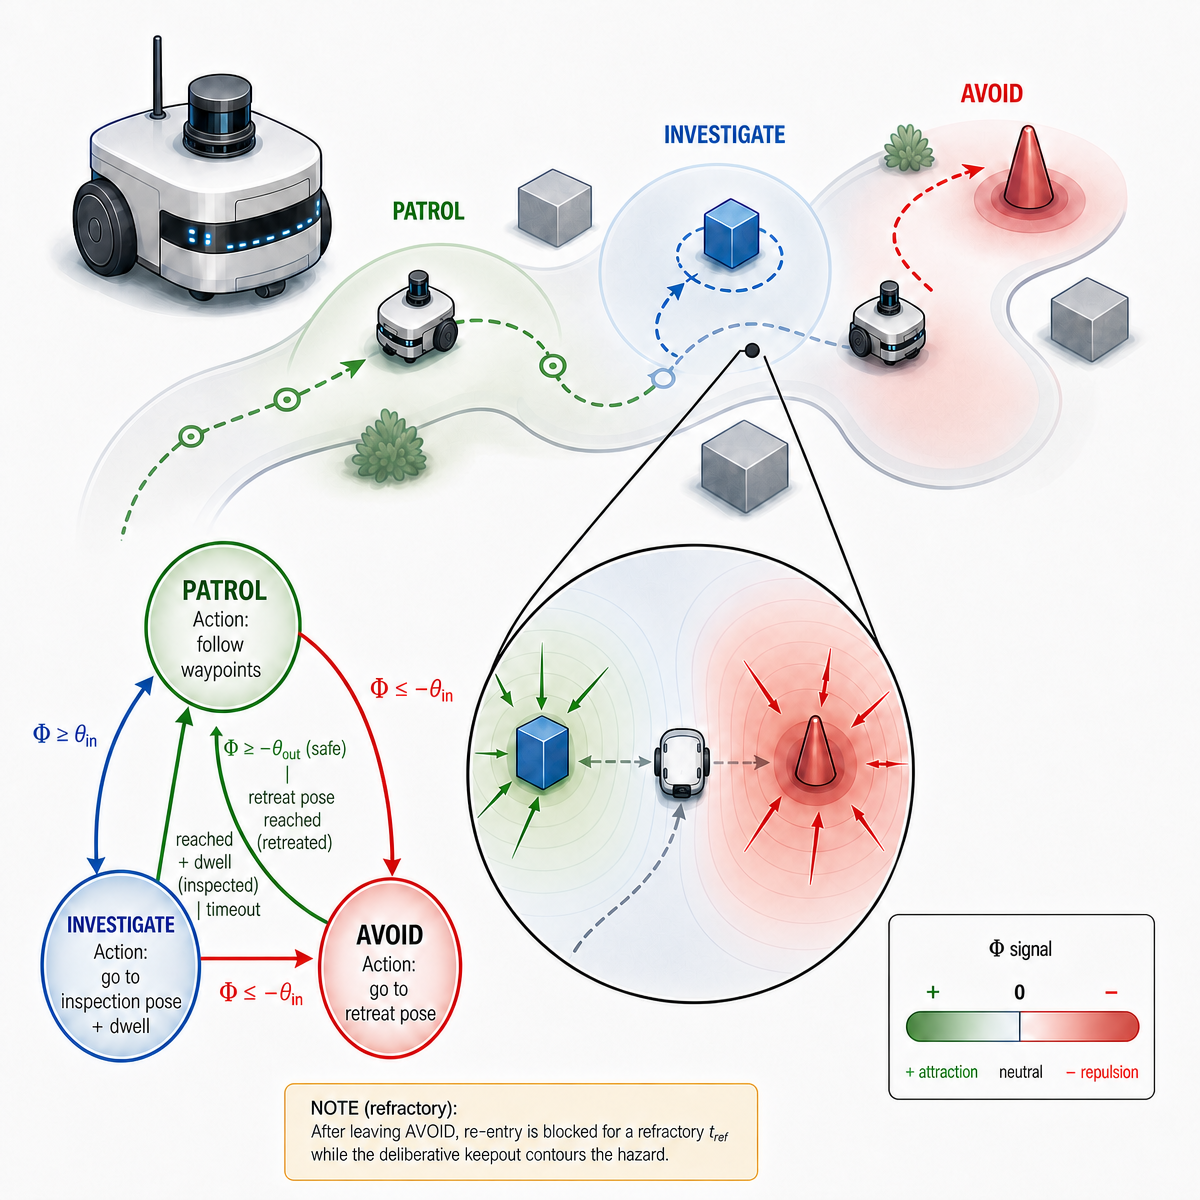
\includegraphics[width=\columnwidth]{stay_alert_fsm}
\caption{\textsc{Stay Alert} state machine and attraction--repulsion field. Top: along the
patrol the robot switches to \textsc{Investigate} (approach an anomaly) or
\textsc{Avoid} (retreat from a hazard). Bottom-left: the three modes and their
transitions ($\theta_{\text{in}},\theta_{\text{out}}$ thresholds; outcomes
\emph{inspected}/\emph{timeout}/\emph{safe}/\emph{retreated}; repulsion has
priority). Bottom-right: the field pulls toward attraction (green) and
pushes away from repulsion (red).}
\label{fig:fsm}
\end{figure}

\begin{algorithm}[t]
\caption{\textsc{Stay Alert} reactive layer (per control tick)}
\label{alg:stayalert}
\begin{algorithmic}[1]
\STATE \textbf{input:} field $\Phi$; selected event $e^\star$ (most salient in
       range); thresholds $\theta_{\text{in}},\theta_{\text{out}}$;
       $t_{\text{dwell}}, t_{\max}$; refractory $t_{\text{ref}}$
\STATE \textbf{Safety preemption} (a hazard interrupts \emph{any} state):
\IF{mode $\ne$ \textsc{Avoid} \textbf{and} $\Phi \le -\theta_{\text{in}}$
    \textbf{and} retreat pose available \textbf{and} $t \ge t_{\text{avoid}}$}
  \IF{mode $=$ \textsc{Investigate}}
     \STATE exit (\emph{deferred by hazard}); release target $e^\star$
  \ENDIF
  \STATE enter \textsc{Avoid}; pause patrol; send retreat goal; \emph{hand the
         hazard to the deliberative keepout} (its reactive signal is thereafter
         suppressed, to avoid oscillation while the planner contours it)
\ELSIF{mode $=$ \textsc{Patrol}}
  \IF{$\Phi \ge \theta_{\text{in}}$ \textbf{and} inspection pose available}
     \STATE commit target $e^\star$ (by identity); enter \textsc{Investigate};
            pause patrol; send approach goal
  \ENDIF
\ELSIF{mode $=$ \textsc{Investigate}}
  \IF{navigation \textbf{succeeded}, dwelled $\ge t_{\text{dwell}}$, \textbf{and}
      final pose within the confirmation distance of $e^\star$}
     \STATE exit (\emph{inspected}: credit $e^\star$); resume patrol
  \ELSIF{elapsed $\ge t_{\max}$ \textbf{or} navigation aborted/cancelled}
     \STATE exit (\emph{failed}); resume patrol
  \ENDIF
\ELSIF{mode $=$ \textsc{Avoid}}
  \IF{$\Phi > -\theta_{\text{out}}$ \textbf{or} retreat pose reached}
     \STATE exit (\emph{safe}/\emph{retreated});
            $t_{\text{avoid}} \gets t + t_{\text{ref}}$; resume patrol
  \ELSIF{elapsed $\ge t_{\max}$}
     \STATE exit (\emph{timeout});
            $t_{\text{avoid}} \gets t + t_{\text{ref}}$; resume patrol
  \ENDIF
\ENDIF
\end{algorithmic}
\end{algorithm}

\subsection{Active Sensing and Event Abstraction}
\label{sec:method-sensing}
The patrol realizes active sensing by carrying the sensors along the route; the
robot pose used by the reactive layer is taken in the \emph{map} frame (via the
TF tree), so that events, poses and the static map are mutually consistent. The
output of the sensing-and-perception chain is abstracted as \emph{events}
$(\text{modality}, \text{intensity}, \text{position})$, i.e., we model the
\emph{result} of perception rather than raw sensor streams. This is a scoped
simplification appropriate to an \emph{algorithmic} contribution: it isolates
the navigation-and-decision behavior from the (orthogonal) perception problem,
and keeps the evaluation reproducible.

Given an event at position $\bm{e}$ and the robot at $\bm{p}$, with unit
direction $\hat{\bm{u}}=(\bm{p}-\bm{e})/\lVert\bm{p}-\bm{e}\rVert$,
\textsc{Investigate} targets an inspection pose at a standoff $\rho$ facing the
event, $\bm{p}_{\text{insp}}=\bm{e}+\rho\,\hat{\bm{u}}$, while \textsc{Avoid}
targets a retreat pose beyond the detection radius and facing away,
$\bm{p}_{\text{ret}}=\bm{e}+(R+\Delta)\,\hat{\bm{u}}$. Attraction events are
committed once (then stop attracting); hazards are persistent.
